%%%%%%%%%%%%%%%%%%%%%%%%%%%%%%%%%%%%%%%%%%%%%%%%%%%%%%%%%
\section{Algoritmo propuesto}
\label{posing:method}
%%%%%%%%%%%%%%%%%%%%%%%%%%%%%%%%%%%%%%%%%%%%%%%%%%%%%%%%%
\todo{1. Indicar muy brevemente las ventajas de la animación esqueletal alineadas con los objetivos. 2. Indicar porque la técnica clasica no se puede utilizar. La extendemos para anatomía interna. 3. No usamos las técnicas clásicas porque no tiene en cueta la anatomía interna. %2. No entiendo la seguna parte de la frase
}
El objetivo es ser capaz de modificar toda la anatomía interna y externa de un modelo anatómico virtual usando una representación superficial. \new{En el mundo de los gráficos por computador, tradicionalmente, se ha utilizado la animación esqueletal para transformar la superficie de modelos articulados. Aunque permite una animación de modelos complejos en tiempo interactivo, no tiene en cuenta la relación espacial entre tejidos. Por esta razón, se ha diseñado un cauce basado en la animación esqueletal que se extiende para el uso de representaciones volumétricas.} 
%\del{En lugar de utilizar las técnicas clásicas de animación esqueletal, se ha propuesto una nueva manera novedosa de animar anatomías de personajes de manera eficiente, ya que para animar todos los tejidos de forma separada implicaría que habría que realizar las etapas de la animación para cada tejido de manera independiente y que no se podría asegurar que se generaran auto colisiones entre ellos.}

\new{La idea principal que hay detrás del algoritmo propuesto} es de calcular un campo de desplazamientos continuo %\todo{si no es continuo todo lo que dices a continuación no sirve}
en el interior del paciente virtual y utilizarlo para transformar las estructuras internas. Esto permite deformar los tejidos de forma independiente y, aun así, garantizar que estos se muevan solidariamente, asegurando que no se produzcan colisiones.%\del{ solidaria sin necesidad de realizar cálculos independientes y asegurar de esta manera que no se producirá nuevas colisiones.} 
%\todo{cuentalo luego}\del{Además, esta forma de trabajar permite no sólo animar representaciones superficiales, sino que es factible animar modelos volumétricos.}
\todo{Relata la idea principal. Crear el despalazamiento a partir del movimiento de los huesos. 2. Expliar la diferencia enter hueso virtual y tejido oseo. 3. Una vez acabado el parrafo lee toda esta into para que no haya cosas duplicadas. }

\new{La deformación del campo de desplazamientos vendrá dada por el movimiento del tejido óseo. La influencia de uno o un grupo de huesos reales definirá el movimiento del campo y en consecuencia, el del resto de los tejidos mapeados con la representación volumétrica generada a partir de la piel. }

\new{El movimiento del tejido óseo será dirigido por los huesos virtuales. Estos serán creados y ajustados teniendo en cuenta la anatomía real del paciente virtual, construyendo un esqueleto virtual específico. }


\todo{1. todo automático menos la selección de la pose. 2. Indicar que la animación tradicional confía en el artista en muchos paso}
\new{En la industria, es el animador el que se encarga exclusivamente de los movimientos de los personajes, confiando en sus habilidades. Otro de los objetivos propuestos para este algoritmo es permitir a un médico dirija y supervise la deformación del paciente virtual de manera interactiva. A su vez, puede guardar posturas interesantes que permitan animar los modelos automáticamente en un futuro.
Se ha buscado en la bibliografía aquellas técnicas automáticas que puedan ser útiles como se puede leer en el estado del arte (sec. \ref{art:anatomy}) y se han adaptado para ser incorporadas en este método con el objetivo de reducir la interacción del usuario a la selección de pose.
%o dejará la elección de la postura a un profesional médico que supervise la correcta deformación de los tejidos de forma interactiva.
} 

%Como se ha especificado en la sección \ref{posing:req}, esta técnica ha sido diseñada para funcionar con anatomías incompletas siendo sólo obligatorio que la piel y los huesos estén correctamente identificados. \todo{1. Esta frase no se como se enlaza con la anterior. 2. repites la idea de etapas automaticas que ya habías explicado en el paso anterior.}\todo{aqui te quedaste}%El algoritmo propuesto sigue la línea del cauce clásico de animación esqueletal, modificando aquellas etapas con el objetivo de que sea automático y permita modelos incompletos.

%\del{Por tanto, el algoritmo propuestose puede dividir en las siguientes etapas}. 
\new{A continuación se detallan las etapas en las que se divide el algoritmo} (ver Fig. \ref{fig:Resumen}). \new{Tal y como puede comprobarse, muchas de las etapas, se inspiran en la animación esqueletal tradicional}:
\todo{Déjalo en ingles, pero en el estado del arte, cuando se hable de rigging, mete un nota al pie donde digas lo que es. Hecho }
\begin{itemize}

	\item \emph{Rigging}: %\todo{Se que has traducido del ingles, pero tio!!! que tu hablas castellano} \del{Un esqueleto virtual predefinido \del{es} ajustado a la anatomía del personaje.}
	\new{En la primera etapa, se adapta un esqueleto virtual a la anatomía del paciente virtual.} El algoritmo usa el tejido óseo para calcular el centro de rotación de cada articulación (sec. \ref{art:rigging}) del hueso virtual.
	
     \item \emph{Volumetrización}: En esta etapa, se genera una malla de tetraedros que volumetriza el interior del modelo. Esta malla se genera a partir de la de la piel y los huesos del paciente virtual y servirá para definir un campo de desplazamientos continuo, que se asociará con el movimiento de los huesos.
\item \emph{Pesado}: A continuación, se calcula de manera automática la influencia del tejido óseo a cada vértice de la malla de tetraedros. 
\item \emph{Mapeado}: Todos los demás tejidos son asignados a los tetraedros de la malla volumétrica. 
\item \emph{Selección de pose}: En esta etapa, el movimiento de los huesos virtuales es transferido a la malla de tetraedros usando una técnica estándar de \emph{skinning}: \ac{LBS}, \ac{DQS} o \ac{COR}. 
%\todo{Esto no es la primera vez que te lo digo. Cuando utilices la pasiva que suene natural!!!}
Después, el movimiento de estos tetraedros se transferirá aplicado a los tejidos del resto del modelo. Esta etapa puede ser interactiva dejando al usuario elegir la pose, o puede usarse otras técnicas de animación (p.ej. \ac{MoCap}) con el objetivo de que la etapa se ejecute de manera automática.%\todo{La cinemática inversa no es automática, es interactiva. }
\item \emph{Optimización}: De forma opcional,
\new{ el usuario podrá refinar el resultado obtenido utilizando un método que intente preservar el volumen del modelo anatómico.}
\todo{La frase es rara. Creo que con la intención  no suena bien.}
\del{De forma opcional, se permite al usuario refinar el resultado obtenido con \new{la finalidad} \del{la intención }de preservar el volumen del modelo anatómico.}

\end{itemize}

%\todo{rehacer imagen resumen}
%\todo{hazla más grande}
\begin{figure*}[!th]
   \centering
    \includegraphics[width=0.95\textwidth]{IMG/resumen.eps}%[width=0.95\textwidth]
    \caption{Perspectiva general del algoritmo propuesto}
		\label{fig:Resumen}
\end{figure*}


%

A continuación, se describirá detalladamente cada una de las etapas por separado, remarcando aquellas innovaciones y adaptaciones hechas específicamente para esta solución.



%%%%%%%%%%%%%%%%%%%%%%%%%%%%%%%%%%%%%%%%%%%%%%%%%%%%%%
\subsection{Rigging}
\label{posing:rigging}
%%%%%%%%%%%%%%%%%%%%%%%%%%%%%%%%%%%%%%%%%%%%%%%%%%%%%%
De manera similar a los huesos reales, un esqueleto virtual permite el movimiento del personaje que se quiere animar. El esqueleto virtual se representa como un conjunto jerarquizado de huesos virtuales conectados entre sí. El movimiento de cada hueso virtual está definido por una rotación teniendo en cuenta el centro de rotación de la articulación. Este movimiento puede ser fácilmente ampliable a otros tipos de movimientos más complejos discutidos en la sección \ref{art:rigging}. \new{De la misma manera, se han mencionado varias formas de crear o ajustar un esqueleto virtual a un modelo de entrada.}

\new{En esta etapa, se ha optado por crear un procedimiento por el cual se ajusta un esqueleto virtual predefinido al tejido óseo del paciente virtual. Se utiliza la propia representación superficial del tejido para definir un centro de rotación y los ejes cartesianos para cada articulación.}
\todo{
%1. Explica que en la bibliografia existen técnicas que crean en el esqueleto y otras que ajustan uno existente. 
2. En Rasimas los pacientes se generan registrando datos reales en el modelo del Zygote. 
3. Redacta lo que viene a  continuación para que este bien ligado con esto. 
4. Tienes que encuenta que etiquetas el modelo en reposo. %Recuerda el documento que nos pasó antoine. De hecho puedes poner este docuemento en el apendice y citarlo. 
De verdad falta mucha información}

\new{Para ello, se han identificado manualmente las regiones significativas de cada hueso o conjunto de huesos, a partir del cual se calculará el sistea local de referencia del hueso virtual. En la figura \ref{fig:humero}, se pueden apreciar las distintas regiones seleccionadas para una muestra de diferentes huesos. Las zonas rojas sirven para calcular el centroide que se usará como punto de rotación para los huesos virtual. Con este punto y los centroides obtenidos de las áreas de color azul y verde se puede estimar dos vectores ortogonales: un vector vertical entre la zona roja y verde; y otro vertical entre la zona verde y azul. El tercer eje se calcula mediante el producto vectorial de ambos. Estos vectores servirán para definir el sistema local de referencia para esa articulación.}

\new{Estas zonas etiquetadas se identifican en el modelo anatómico de entrada. Inicialmente, en el proyecto \ac{RASimAs}, se utiliza el modelo \emph{ZygoteBody}$^{TM}$, pero se puede asumir que el modelo de entrada en la herramienta \ac{ITGVPH} se puedan identificar las mismas regiones.} Además, para hacer estos cálculos más robustos, el algoritmo considerará (cuando sea posible) regiones más grandes, minimizando los posibles defectos de un mal registro. Este proceso es específico para cada hueso virtual y puede ser fácilmente ampliable para todo tipo de huesos. La explicación de cada hueso que se ha utilizado en la presente tesis se podrá consultar en el anexo \ref{anexo:rigging}. 
\todo{Creo que tienes que mejorar como enlazas las ideas en este parrafo.}
Esta etapa concreta ha sido desarrollada por \emph{Antonie Serruier}, miembro del proyecto \ac{RASimAs}, en colaboración con el autor de esta tesis basada en anteriores trabajos \cite{QUIJANO20131703}.
\todo{revisar los colores de las fotos}
\todo{Aumenta el tamño de todas las imágnes}

\todo{indica el código de colores}
\begin{figure}
   \centering
    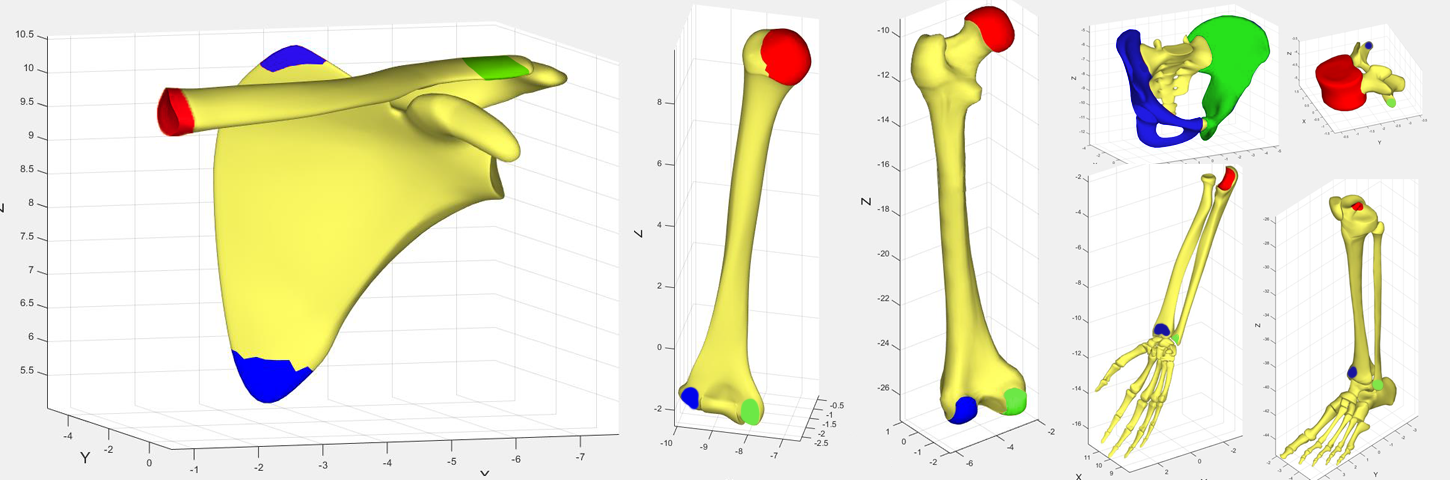
\includegraphics[width=0.95\textwidth]{IMG/rigshoulder.png}%[width=0.8\textwidth]
    \caption{La imagen muestra los huesos del modelo de referencia antes de registrar los datos del paciente. Las áreas coloreadas se utilizan para calcular el sistema de referencia de cada articulación. \new{El centro de rotación se calcula a partir de las zonas rojas. Dos vectores ortogonales se calculan con las zonas azul y verde. El tercero se calcula en base a los dos anteriores.}}
\label{fig:humero}
\end{figure}


%%%%%%%%%%%%%%%%%%%%%%%%%%%%%%%%%%%%%%%%%%%%%%%%%%%%%%
\subsection{Volumetrización}
\label{posing:volumetrizacion}
%%%%%%%%%%%%%%%%%%%%%%%%%%%%%%%%%%%%%%%%%%%%%%%%%%%%%%
%
Como se ha introducido anteriormente, \new{el objetivo es crear un campo de desplazamientos continuo que permita mover la anatomía interna del paciente virtual}. El algoritmo discretiza el interior del modelo utilizando la piel y el tejido oseo como referencia, obteniendo una malla volumétrica formada por tetraedros. Esta malla de tetraedros es una pieza clave del algoritmo que se utilizará para calcular el citado campo de desplazamientos. La siguiente etapa (sec. \ref{posing:Pesado}) calculará la influencia del movimiento de cada hueso en los vértices de los tetraedros, de forma que el movimiento de los huesos afecte a los vértices de la malla volumétrica. El campo de desplazamientos se obtendrá de forma implícita interpolando el desplazamiento de los vértices en el interior de los tetraedros, mediante el uso de coordenadas baricéntricas. \new{Esta malla será fundamental en las siguientes etapas.}
%\del{Después, esta malla será donde se calcule el campo de desplazamiento (Sec. \ref{posing:Poses}). También, el campo de desplazamientos guiará la animación del modelo virtual gracias al cálculo del mapeado entre los tetraedros generados en esta etapa y los distintos tejidos (Sec. \ref{posing:Mapeado}).}  \todo{Estas ultimas frases son muy raras, sobretodo la final. Explicas cosas que no son necesarias para esta etapa. }


%\todo{No te das cuenta de confusa que es esta frase. Lo que quieres decir es que no calculas directamente la malla de tetraedros, primero creas una imagen volumétrica. Reescribe}
%\del{En lugar de proceder al proceso de discretización con las representaciones superficiales de los tejidos, se ha optado \new{por} generar una representación volumétrica a partir de la piel y los huesos como paso intermedio para controlar el proceso de discretización y mejorar la robustez del algoritmo. Se genera una imagen en tres dimensiones compuesta por \emph{vóxeles}\footnote{unidad cúbica mínima para representaciones volumétricas} que permitirá simplificar el etiquetado aquellos \emph{vóxeles} que \del{colisionan con} \new{pertenezcan a} la piel y los huesos.}\todo{simplificar?}
\new{ La malla volumétrica no se realiza de forma directa, sino que se ha decidido general una representación superficial a partir de la piel y los huesos como paso intermedio para controlar el proceso de discretización y mejorar la robustez del algoritmo. Se genera una imagen en tres dimensiones compuesta por} \emph{vóxeles}\footnote{unidad cúbica mínima para representaciones volumétricas}\new{  que permitirá simplificar el etiquetado aquellos que pertenezcan a la piel y los huesos. }

El tamaño de la imagen 3D depende de los tamaños del \emph{vóxel} y de la caja contenedor del modelo. Cuanto más grande sea dicha caja y el tamaño del \emph{vóxel} más pequeño, más detalle tendrá la imagen 3D resultante. \new{Sin embargo, hay que tener en cuenta que a más detalle, más tiempo de cálculo y más consumo de memoria será necesario.}%\todo{revisa la frase anterior}
En esta tesis se ha establecido un tamaño de \emph{vóxel} que permita tener como máximo una caja contenedora de tamaño 250x700x120.

El proceso de \emph{voxelización} empieza etiquetando aquellos \emph{vóxeles} que coinciden con la piel (Fig. \ref{fig:voxelizacion}.a). Después, los \emph{vóxeles} interiores se etiquetan usando la técnica descrita en \cite{SUZUKI20031} (Fig. \ref{fig:voxelizacion}.b).\todo{expresalo de otra manera}\new{ En este punto, se ha decido añadir una etapa donde aquellos \emph{vóxeles} que pertenecen a la superficie de la piel vuelven a estar no etiquetados \del{como vacíos}}(Fig. \ref{fig:voxelizacion}.c). Este paso se ha introducido para mejorar la robustez del método en zonas que podrían quedar interconectadas por su proximidad. En el apartado de resultados se mostrará la motivación de esta etapa. Finalmente, se procede a etiquetar los \emph{vóxeles} que corresponden a cada hueso como se muestra en la imagen (Fig. \ref{fig:voxelizacion}.d), de forma similar al procedimiento que se utiliza con la piel. 
%
%\todo{puedes hacer la imagenes más grandes. No hay limite de espacio!}
%
\begin{figure}[th]
   \centering
    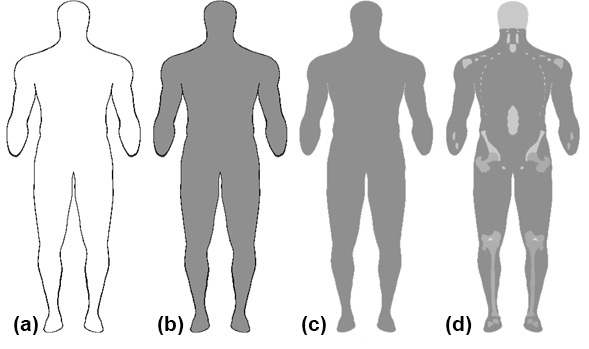
\includegraphics[width=0.95\textwidth]{IMG/Volume2.png}
    \caption{
    Cortes coronales de la imagen volumétrica en las distintas etapas del proceso de \emph{voxelización}.}
\label{fig:voxelizacion}
\end{figure}

\todo{me gusta esta separación. Usala en el texto. Fase 1 voxelización, fase tetraedrización}
Una vez que la imagen 3D ha sido construida, se utiliza para crear una malla de tetraedros asociada. Para la tetraedrización se utiliza el algoritmo \ac{RDT} \cite{jamin:hal-00796052}. Este algoritmo permite generar mallas de tetraedros multidominio a partir de mallas superficiales o imágenes 3D. A la hora de configurar el algoritmo, se debe alcanzar un compromiso entre precisión y eficiencia (ver anexo \ref{anexo:criterios}). Se ha configurado para incrementar los tetraedros alrededor de la piel y la superficie de los huesos. Para la realización de esta tesis, se ha conseguido mantener el número de los tetraedros por debajo de $3.5\times 10^6$ y el número de vértices por debajo de $8 \times 10^5$. Destacar que la malla de tetraedros se etiquetada usando los tejidos óseos y la piel (Fig. \ref{fig:tetra}).
%
\begin{figure}[th]
   \centering
    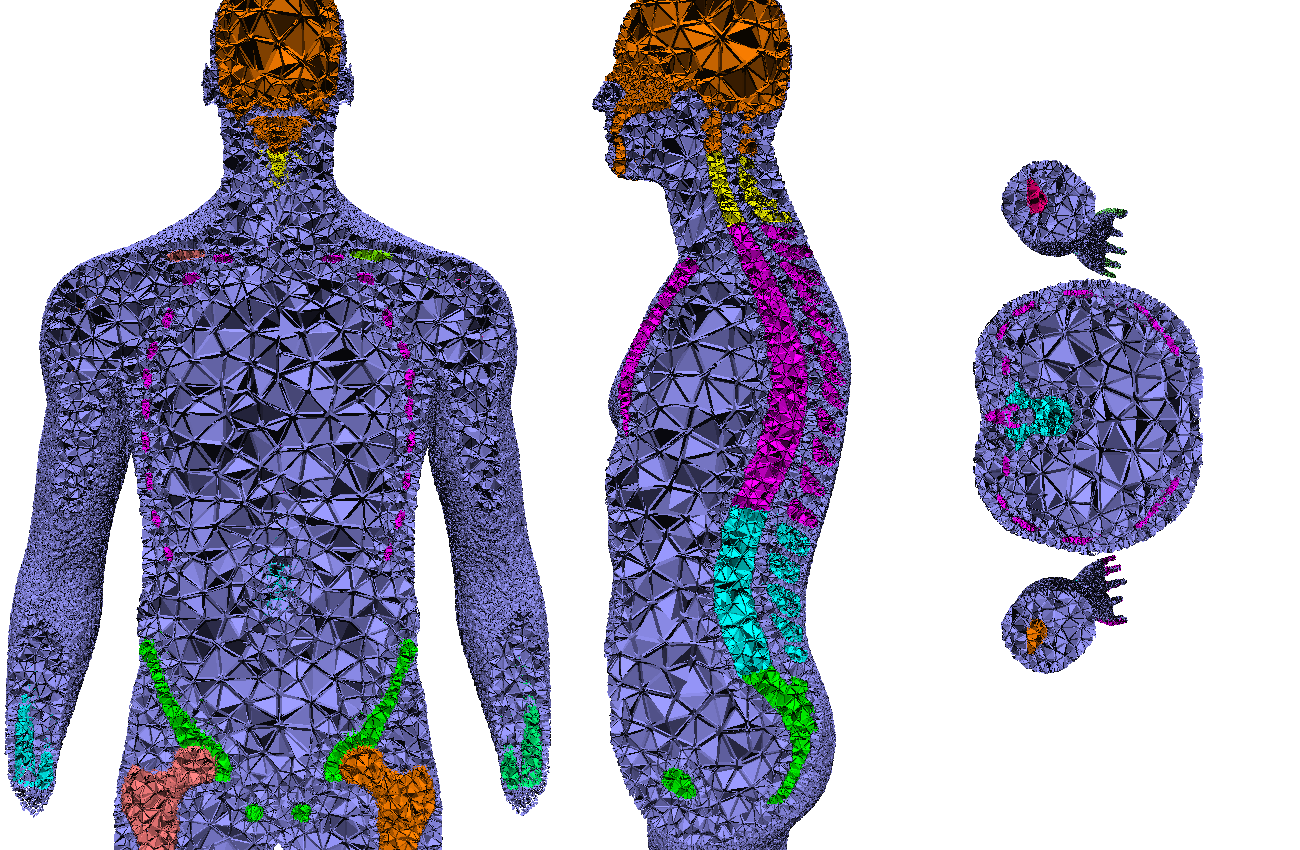
\includegraphics[width=0.95\textwidth]{IMG/boneid.png}
     \caption{Cortes coronales, sagitales y axiales mostrando el resultado de la tetraedrización. Los tetraedros etiquetados como huesos se muestran en diferentes colores.}
\label{fig:tetra}
\end{figure} 

%%%%%%%%%%%%%%%%%%%%%%%%%%%%%%%%%%%%%%%%%%%%%%%%%%%%%
\subsection{Pesado}
\label{posing:Pesado}
%%%%%%%%%%%%%%%%%%%%%%%%%%%%%%%%%%%%%%%%%%%%%%%%%%%%%%
%
Como se ha introducido en el estado del arte (ver sección \ref{art:pesado}), la etapa de pesado es donde se calcula como influye el movimiento de cada hueso sobre los vértices de la malla superficial. \new{Es habitual encontrar que las técnicas citadas están orientadas al pesado en mallas superficiales. Sin embargo, como se están tratando con mallas de tetraedros, hay que adaptar estos modelos a la problemática presente. }
%\todo{En el paso anterior no se calculó un campo de desplazamientos. Volumetrizó el espacio interior. El pesado calcula la influencia de los huesos sobre los vértices. Esta influencia se usa para mover los vértices siguiendo el movimiento de los huesos. Una ve que se han movido los vértices se calcula el campo de desplazamientos en el interior de cada tetraedro interpolando mediante coordenadas baricéntricas el desplazamiento de los vértices. En resumen la frase es confusa cambiala}.
\new{A su vez, tampoco se desea calcular la influencia del esqueleto virtual, sino calcular como se propagan la influencia de los tejidos óseos sobre los demás vértices de la malla de tetraedros.}
%\del{Así pues, en este caso se va a calcular la influencia de los huesos reales y no de los huesos virtuales a los vértices de la malla de tetraedros y no de los vértices de los distintos tejidos}
%\todo{Separa las ideas. La primera diferencia es que no se usa el esquelto virtual, sino que se propaga la influencia del tejido oseo. Diferencia 2, no se calcula la influencia sobre el resto de tejidos sino que se calcuala la influencia sobre los vertices de la malla volumetrica}. 


Al igual que los algoritmos de pesado clásicos, los pesos calculados para los vértices de los tetraedros tienen que cumplir las mismas condiciones que se citan en \ref{cond1} y \ref{cond2}.
\emph{Baran y Popovi\'{c}} en \cite{Baran:2007} presentan un trabajo que realiza el pesado de forma automática y crea transiciones suaves entre articulaciones. Ellos proponen usar la ecuación de difusión de calor suponiendo que la influencia de los huesos se propaga a través del modelo al igual que haría el calor. %Existen actualmente técnicas para calcular el pesado de forma más efectiva \cite{Jacobson:2011} comentadas en el estado del arte, pero se basan en el mismo principio\todo{que no se basen en el mismo principio no es suficiente para descartarlas}. 
%Tomando en cuenta la idea original de \emph{Baran y Popovi\'{c}}\cite{Baran:2007}, se ha modificado\todo{que se ha modificado} para adaptarla al algoritmo propuesto debido a que su aplicación no es directa\todo{reescribe la frase}.

\new{Esta técnica esta diseñada para mallas superficiales y, por tanto, es necesario que se adapte para poder aplicar la propagación de la influencia del tejido óseo al resto de los tetraedros de la malla volumétrica.
%\todo{1. Rehaz la pasiba.}. 
En \cite{Baran:2007}, se resuelve la ecuación del calor \ref{diffusion}donde se hace una analogía entre temperatura y el peso de los vértices. }
\begin{equation}
\label{diffusion}
 \frac{\delta T}{ \delta t} = k \Delta T + q_{G}.
\end{equation}
\todo{revisar}

\new{Asumiendo que no hay fuentes de calor, se ha formulado el caso estático para cada hueso, esto es igualar a cero el operador laplaciano. Esto da lugar a la ecuación \ref{ourdiffusion}}:
\begin{equation}
\label{ourdiffusion}
\Delta W_j = 0.
\end{equation}

%De esta forma, se obtiene un campo de pesos $W_j$  para cada hueso donde el tejido óseo correspondiente a $j$  propaga su influencia (temperatura 1) en el que se está resolviendo e influencia nula (temperatura 0) para el resto de huesos.  %de forma que la solución propuesta hace que la energía laplaciana sea estacionaria. Además, esta adaptación asegura una suavidad de orden superior\todo{la frase no suena bien}. 
\todo{reescribe la frase. Da la sensación que no entiendes que escribes.: flojeo un poco en esta parte sobre todo al escribirla 1 Reformulamos el problemas haciendo cero el laplaciano. Esto es equivalente a minizar la energia. }
%


%Con el objetivo de calcular  de un hueso $j$, se resuelve el caso estacionario definido en la ecuación \ref{diffusion}.%\todo{Tengo la impresion de que sueltas frases sin preocuparte de que sigan un orden logico. Esto está muy flojo.}
\new{Para calcular los pesos $W_j$, esta ecuación se resuelve para cada hueso $j$, donde se imponen las siguientes condiciones de contorno: se considera que el valor $W_j$ es $1$ (influencia) dentro de los tetraedros etiquetados como $j$; y el valor es $W_j$ es $0$ (influencia 0) dentro de los tetraedros etiquetados como $k$, donde $k$ es cualquier otro hueso que no es $j$. En el equilibrio estático, el resto de vértices tienen que verificar la ecuación \ref{ourdiffusion}. El problema se define de la siguiente manera:}

\begin{equation}
\label{problema1}
\Delta W(x)_{j} = 0 \\
\end{equation}
\begin{equation}
\label{problema2}
W(x)_{j} = 1\ \;
\forall x \in B_{j} \\
\end{equation}
\begin{equation}
\label{problema3}
W(x)_{j} = 0\ \;
\forall x \in B_{k}; k\neq j
\end{equation}

\new{donde $W$ es el campo de pesos definido en el dominio $x$. $j$ indica el hueso para el que se está resolviendo, mientras que B es el subdominio de $x$ que representa el hueso real.}

%
\new{Dado que las condiciones de contorno se imponen directamente sobre la malla de tetraedros, no es necesario definir matrices de visibilidad que transfieran el calor desde los huesos virtuales a los vértices como ocurría en \cite{Baran:2007}. En comparación, a un mayor número de vértices perteneciente a la malla de tetraedros, el sistema de ecuaciones resulta mucho mayor.}
\new{Con el objetivo de resolver la ecuación \ref{problema1}, se discretiza usando \ac{FEM} y se utilizan las coordenadas baricéntricas de los tetraedros como función de forma (ver \cite{Lewis2004}). La ecuación \ref{system} muestra la discretización final de la ecuación de difusión:}
%
\begin{equation}
\label{system}
\mathbf{A} \mathbf{W}_j = \mathbf{b}_j,
\end{equation}
%
donde $\mathbf{A}$ es la matriz de coeficientes del sistema, el vector $\mathbf{b}_j$ depende de las condiciones de contorno del hueso  $j$ y $\mathbf{W}_j$ es un vector que  contiene los pesos  $w_{i,j}$ para cada vértice sin etiquetar $i$. \new{$\mathbf{A}$ es constante para todos los huesos ya que solo depende de la discretización del dominio. Como esta matriz es simétrica y definida positiva, permite calcular la descomposición de \emph{Cholesky} de esta matriz una única vez y usarla para resolver el sistema lineal de cada hueso.}

Es importante mencionar que esta formulación cumple con las restricciones que se imponen en \ref{cond1} y \ref{cond2}. \new{Primero, se puede asegurar que el valor máximo y mínimo sólo se alcanzan en los huesos (influencia $0$ o $1$). Segundo, si se considera \ref{min1}  y  \ref{min2}, donde  $n$ es el número de huesos, el sistema \ref{min3} equivale a calcular los pesos donde todos los puntos del contorno tendrán un valor de $1$. Además, como el máximo y el mínimo valor es alcanzado solamente en el contorno, dará lugar a que el valor de la suma de los pesos $\mathbf{W}$ será $1$, probando la condición \ref{cond2}.}

\begin{equation}
\label{min1}
b = \sum^{n}_{j=0} b_{j} 
\end{equation}
\begin{equation}
\label{min2}
W = \sum^{n}_{j=0} W_{j} 
\end{equation}
\begin{equation}
\label{min3}
A W = b
\end{equation}

Existen alternativas como se puede leer en la sección \ref{art:pesado}, donde \cite{Jacobson:2011} presentaba una técnica que permitía crear puntos de anclaje y cajas contenedoras para controlar la animación. Esto daba lugar a resolver un problema disperso y cuadrático para imponer las restricciones. Sin embargo, la solución propuesta en esta sección solo requiere resolver un sistema de ecuaciones lineales. %\nuevo{revisar Marcos. No suena bien. Pero no te lo puedo reescribir todo.}
 %Por otra parte,  mientras que la técnica


 \begin{figure}[h]
   \centering
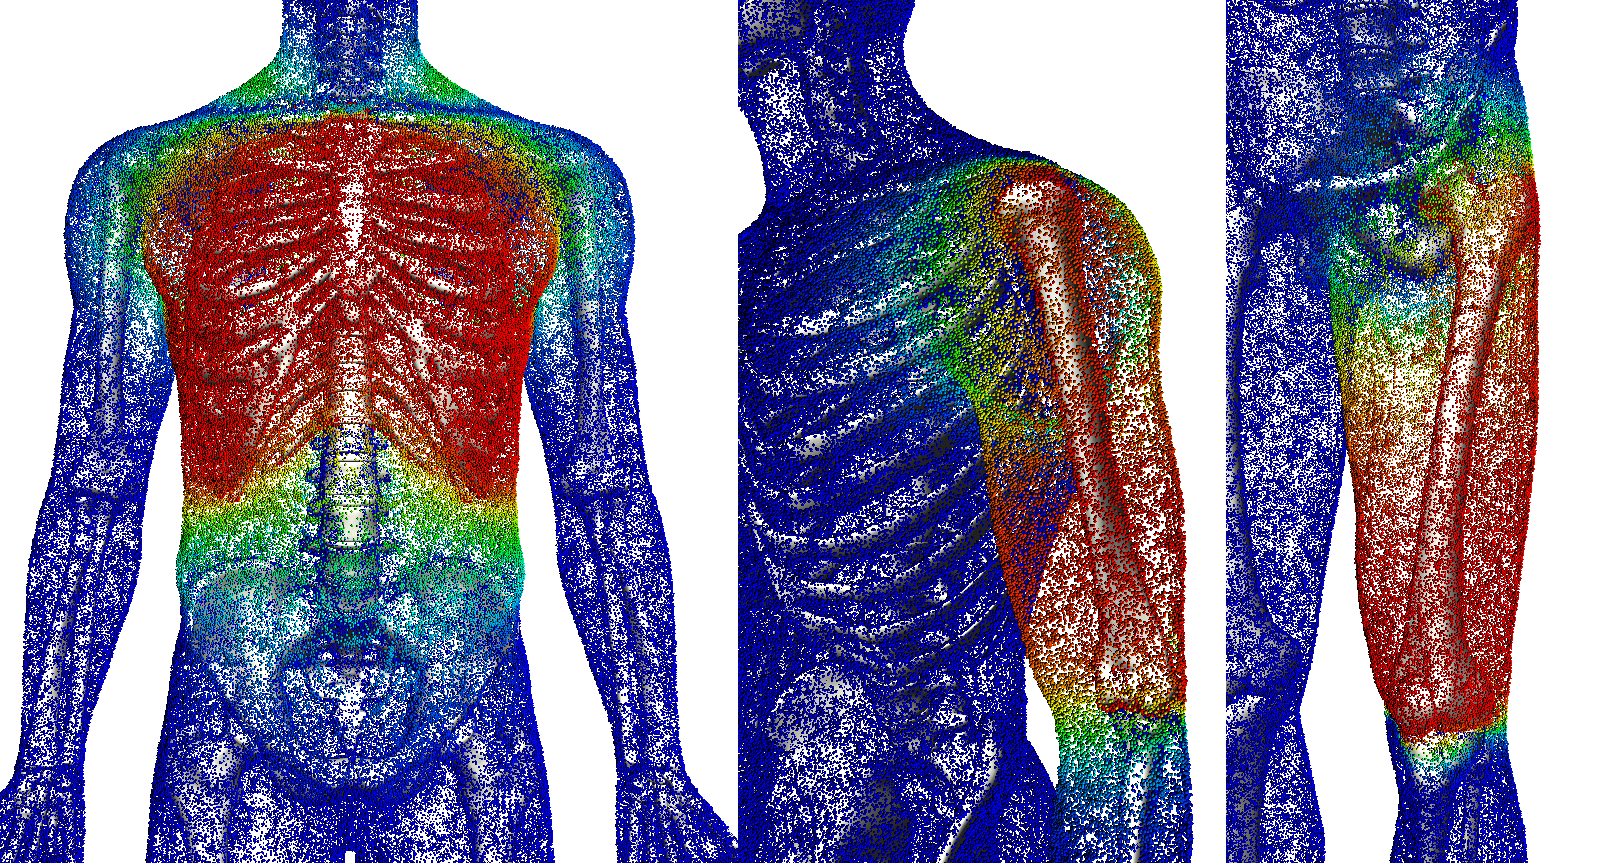
\includegraphics[width=0.49\textwidth]{IMG/weights.png}
     \caption{\new{Vértices de la malla de tetraedros que muestran la influencia de cada hueso o conjunto de huesos. Rojo significa peso cercano a 1 y el azul cercano a 0.}}
      \label{fig:pesado}
\end{figure}
 
Como resultado del desarrollo, en la figura \ref{fig:pesado} se observa como ejemplo la influencia de la caja torácica, el húmero y el fémur en los vértices de la malla de tetraedros. Las zonas rojas muestran valores de influencia cercanos a 1 y las zonas azules cercanas a 0. 






%%%%%%%%%%%%%%%%%%%%%%%%%%%%%%%%%%%%%%%%%%%%%%%%%%%
\subsection{Mapeado}
\label{posing:Mapeado}
%%%%%%%%%%%%%%%%%%%%%%%%%%%%%%%%%%%%%%%%%%
%
Para poder transferir los movimientos de las articulaciones virtuales a los tejidos del modelo, hace falta relaciona cada vértice de las mallas superficiales con un tetraedro. Esto consigue que el campo de desplazamientos definido por la malla de tetraedros sea trasladado a todos los tejidos que se pretendan animar.\todo{Tus frases no suenan naturales}

Se puede parametrizar la posición del vértice que ocupa dentro de su tetraedro asociado con ayuda de las coordenadas baricéntricas. Estas coordenadas indican la influencia de cada uno de los vértices del tetraedro al vértice que esta mapeado. Por tanto, hay que calcular cada una de las coordenadas baricéntricas para cada vértice de las mallas superficiales.

El enfoque más simple es comprobar cada $n$ vértices con cada $m$ tetraedros. Eso significa que la complejidad de comprobar uno a uno es de $\mathcal{O}(n\ m)$. Para acelerar el cálculo global, se ha utilizado la técnica \emph{Spatial Hashing}\cite{Teschner2003}. \new{Esta técnica subdivide el espacio en regiones cúbicas, y se introducen los tetraedros que esten dentro de ese espacio en una \ac{tabla hash} que permite un acceso de complejidad $\mathcal{O}(1)$. En vez de comprobar si el vértice esta dentro de un tetraedro uno por uno, esta técnica permite comprobar solo aquellos tetraedros que se encuentran en la misma subdivisión espacial.  De esta manera se ha reducido el tiempo que tarda el método de fuerza bruta desde horas a menos de un minuto. En el caso de que algún vértice quedará fuera de la malla de tetraedros, la misma \ac{tabla hash} puede facilitar la búsqueda del tetraedro más cercano en las regiones adyacentes.}
%\todo{No esta bien explicado}


%%%%%%%%%%%%%%%%%%%%%%%%%%%%%%%%%%%%%%%%%%%%%%%%%%%%%%
\subsection{Selección de poses}
\label{posing:Poses}
%%%%%%%%%%%%%%%%%%%%%%%%%%%%%%%%%%%%%%%%%%%%%%%%%%%%%%
%
En esta etapa, el usuario es el encargado de seleccionar interactivamente la posición que se quiera trasladar al personaje virtual. El algoritmo desarrollado en esta tesis permite usar cinemática directa, poses pregrabadas y animaciones, incluso usar el dispositivo \emph{Microsoft Kinect}~\cite{shotton2013} para capturar la pose del usuario y transferirla al paciente virtual. Aun así, técnicas como \emph{retargeting} \cite{7581666} o cinemática inversa, podrían ser añadidas en el futuro. %ser incluidas en el algoritmo.
\todo{el pueden ser incluidas suena mal.}

Para transferir la animación esqueletal a una malla superficial se utilizan diferentes algoritmos de \emph{skinning} (ver sec.\ref{art:skinning}).
%\todo{el skinning no es un modelo matematico, son los algoritmos que transfieren el movimiento de los usos... Tal y como esta redacto parece que en el estado del arte has anticipado que TU ALGORITMO USARA EL SKINNING}.

%En el caso del algoritmo propuesto, se puede tratar los vértices de los tetraedros como vértices de una malla superficial\new{????}. De la misma manera que la animación clásica las animaciones esqueletales son transferidas a la malla volumétrica usando una técnica de \emph{skinning}. Los tetraedros deformados definen un campo de deformación que se utiliza para animar todos los tejidos del paciente virtual.
\new{En el caso del algoritmo propuesto, las técnicas de  \emph{skinning} se aplicarán a los vértices de la malla de tetraedros. Los vértices del resto de tejidos del modelo serán transformados gracias al campo de desplazamientos. Este se obtendrá de forma implícita interpolando el desplazamiento de los vértices en el interior de los tetraedros. Mediante el uso de coordenadas baricéntricas, se traslada el movimiento de los tetraedros a los vértices de todos los tejidos del paciente virtual.}

%\todo{A partir de ahora solo voy a dar pinceladas. Llevo la mañana del viernes, la del sabado y la del domingo y no avanzo. No puedo comentar cada frase. Es TU RESPONSABILIDAD cuidar la redacción. }


Se ha elegido implementar la técnica de \emph{skinning} descrita en \cite{le2016real}. \new{Se ha decidido usar la técnica \ac{COR} ya que resuelve algunos de los problemas de \ac{DQS} y \ac{LBS} descritos en la sección\ref{art:skinning}.} \emph{Le y Hodghins} calcula unos centros de rotación óptimos para todos los vértices de la malla. %En este caso, es necesario  de tetraedros\todo{paredce que son ellos trabajan con mallas de tetrahedros}. 
Una vez esta información es calculada, esta técnica no afecta al rendimiento del sistema en comparación con las técnicas más utilizadas \ac{LBS} y \ac{DQS}. %Estas tres técnicas son intercambiables entre si debido a que están perfectamente diseñadas para usarse con las arquitecturas gráficas modernas.
Este algoritmo se basa en que los vértices con un pesado similar deben seguir las mismas transformaciones que sus vecinos. \new{En su trabajo, \emph {Le y Hodgins} ~\cite{le2016real} proponen una función de similaridad con la que ponderar la contribución de los vecinos según lo parecidos que sean los pesos. Con la finalidad de adaptar la formulación de una malla de triángulos a una malla de tetraedros, se van a mostrar a continuación todos los cambios realizados:}
%\todo{pasivas, intercambiables????}

%\begin{eqnarray}\nonumber
\begin{equation}
 s(\textbf{w}_p,\textbf{w}_s) = 
\sum_{\forall i \neq j} w_{p,i}w_{p,j}w_{s,i}w_{s,j}\exp-\frac{(w_{p,i}w_{s,j}-w_{s,i}w_{p,j})^2}{\sigma^2}
\end{equation}
%\end{eqnarray}
\normalsize
%
donde $\textbf{w}_p$ y $\textbf{w}_s$ son vectores de los pesos de los vértices $p$ y $s$, y $\sigma$ parametriza la función exponencial. El valor de $\sigma$ que se utiliza es $0.1$ .Esta función se usa para calcular el nuevo centro de rotación. \new{De la misma manera, es necesario adaptar la ecuación propuesta en \cite{le2016real} para calcular los centros de rotación. En la ecuación se utiliza la función de similitud anteriormente citada pero teniendo en cuenta que un vértice ahora tendrá los cuatro vecinos que forman el tetraedro. También se intercambia el área del triángulo por el volumen del tetraedro vecino. Así la ecuación se quedará de la siguiente manera}: 
%
\begin{equation}
%\begin{eqnarray}\nonumber
\textbf{cor}_p = 
\frac
  {
  \sum_{\forall t \in T}
    s(\textbf{w}_p,
      \frac{\textbf{w}_{t1}+\textbf{w}_{t2}+\textbf{w}_{t3}+\textbf{w}_{t4}}{4})
    %\frac{\textbf{v}_{t1}+\textbf{v}_{t2}+\textbf{v}_{t3}+\textbf{v}_{t4}}{4}
    V_t\mathbf{c}_t
  }
  {
  \sum_{\forall t \in T}
    s(\textbf{w}_p,
      \frac{\textbf{w}_{t1}+\textbf{w}_{t2}+\textbf{w}_{t3}+\textbf{w}_{t4}}{4})
    V_t
  } 
%\end{eqnarray}
\normalsize
\end{equation}
%
donde $\textbf{cor}_p$ es el nuevo centro de rotación del vértice $p$, $t$ es el tetraedro de la malla de tetraedros $T$, $V_t$ es el volumen del tetraedro $t$, $\textbf{c}_t$ es el centroide del tetraedro $t$ y $\textbf{w}_{t1}$, $\textbf{w}_{t2}$, $\textbf{w}_{t3}$ y $\textbf{w}_{t4}$ son los pesos de los vértices del tetraedro $t$. Una vez calculado este centro, se puede usar en la etapa interactiva utilizando el \emph{shader} descrito en \cite{le2016real}.

Finalmente, para animar los vértices de cada malla, el campo de desplazamiento de un punto dentro de un tetraedro se puede calcular interpolando el desplazamiento de cada uno de sus vértices. Se interpola este campo usando las coordenadas baricéntricas de cada tetraedro, ya calculadas en el paso de pesado (sec. \ref{posing:Pesado}). Matemáticamente, el campo de desplazamientos calculado es continuo pero no diferenciable dentro de la malla volumétrica y permite calcular una matriz de transformación constante por cada tetraedro (consultar \cite{Muller2004}). Esta matriz de transformación, perteneciente al tetraedro, se aplica a cada uno de los vértices de la malla superficial asociados al tetraedro. Estos cálculos se realizan en la tarjeta gráfica para mejorar el rendimiento del algoritmo.

\todo{No se si este apartado se entiende lo basta bien. Es muy criptioco. Redactado, a ver que tal}


% %%%%%%%%%%%%%%%%%%%%%%%%%%%%%%%%%%%%%%%%%%%%%%%%%%%%%%
 \subsection{Optimización}
\label{posing:optimizacion}
% %%%%%%%%%%%%%%%%%%%%%%%%%%%%%%%%%%%%%%%%%%%%%%%%%%%%%%
% %

% %

%Los resultados de la etapa previa son visualmente realistas\todo{¿Como lo sabes?}. \ac{COR} reduce el volumen ganado por \ac{DQS} o el volumen perdido por \ac{LBS}\todo{tienes resultados que lo respalden}. Aun así, hay algunos escenarios dónde se produce un cambio apreciable de volumen.El algoritmo propuesto permite al usuario refinar la solución usando un algoritmo basado en físicas
\new{Aunque se haya decidido utilizar un enfoque geométrico, adicionalmente, se ha propuesto utilizar un modelo basado en físicas que permita al usuario refinar el resultado obtenido. Al no disponer de todos los tejidos o de las propiedades mecánicas, el objetivo de esta etapa no es conseguir un solución realista sino, mejorar el aspecto visual del resultado. Sin las descripciones mecánicas de los tejidos, se ha propuesto una solución que busca la conservación del volumen de cada tetraedro}

%se puede decir que todos los tejidos están compuestos de agua y se asume que es un fluido incompresible y por tanto, las deformaciones tienen que permitir la conservación de volumen para cada tetraedro.}


%\todo{ponemos fórmulas que tenías en los comentarios?}
%\todo{Si eres capaz de explicarlo...}


Para resolver la conservación del volumen de cada tetraedro se plantea el siguiente modelo mecánico que se caracteriza por: plantear las ecuaciones del equilibrio estático, emplear el tensor de deformaciones de \emph{Cauchy} y emplear un modelo de elasticidad isotrópico, homogéneo y lineal. \new{Sin embargo, utilizar un tensor de deformación lineal puede introducir deformaciones incorrectas. Debido a su naturaleza lineal, las rotaciones generan distorsiones en la geometría al interpretarlas como deformaciones, produciendo efectos de escalado o abultamientos. Para resolver esta problemática, se utilizará la formulación co-rotacional del \ac{FEM} para resolver el sistema. La volumetrización del modelo (sec. \ref{posing:volumetrizacion}) se utiliza como discretización espacial y las posiciones de los huesos como las condiciones de contorno necesarias para resolver el problema estático. Para más información se puede consular \cite{Muller2004}.} 

\todo{No es el Fem lo que se configura}
\new{Con la intención de controlar el modelo elástico planteado, se utilizan los parámetros \emph{ratio de Poisson} y \emph {módulo de Young}. Para ajustar y garantizar la conservación del volumen se utiliza un valor ligeramente inferior a 0.5 para asegurar la estabilidad numérica. El comportamiento del material elástico se caracteriza utilizando el \emph {módulo de Young}.  En este caso, este parámetro no será especialmente importante debido solo se busca la solución en equilibrio. En este caso será útil elegir un valor con el objetivo de mejorar la estabilidad numérica del sistema. Para ello se ha analizado la matriz de coeficientes del sistema para varios valores del módulo y se ha seleccionado aquel valor que consiga la matriz de coeficientes con menor número condicionante.}

Respecto a la formulación co-rotacional se basa en calcular en una configuración no rotada las fuerzas internas (derivadas de la deformación) y que se usarán después rotándolas a la configuración final \cite{Muller2004}. Primero, es necesario calcular la rotación de los elementos de la malla de tetraedros. Como esta rotación se desconoce, el problema estático se puede resolver de forma iterativa. Se utiliza la deformación seleccionada por el usuario como situación inicial para reducir significativamente el número de iteraciones requeridas para llegar a la solución final.  %(ver Fig. \ref{x}). 

Para conocer los desplazamientos de los vértices de la malla de tetraedros se ha formulado un sistema de ecuaciones lineales. Según las propiedades anteriormente citadas, la matriz de coeficientes del sistema lineal es dispersa, simétrica y definida positiva. Este tipo de sistemas de ecuaciones se pueden resolver utilizando el método del gradiente conjugado \cite{Press2007}. La convergencia de estos métodos se acelera con el uso de pre-condicionadores (ver \cite{hauth2003}) además de utilizar como punto de partida la posición del modelo ya calculado en la etapa de selección de poses. %Para acelerar esta etapa, se utiliza  como solución inicial la posición del modelo ya calculado en la etapa de selección de poses (sec. \ref{posingPoses}), además de emplear un precondicionador de Jacobi.

Finalmente, se utilizarán los desplazamientos realizados por los tetraedros para calcular la transformación que se aplicará a todos los tejidos asociados (ver sec. \ref{posing:Poses}). 



%%%%%%%%%%%%%%%%%%%%%%%%%%%%%%%%%%%%%%%%%%%%%%%%%%%%%%%%%
\section{Detalles de implementación}
\label{posing:preprocess}
%%%%%%%%%%%%%%%%%%%%%%%%%%%%%%%%%%%%%%%%%%%%%%%%%%%%%%%%%

Como se puede leer en la sección \ref{posing:req}, la selección de poses debe ser supervisada por un usuario y por tanto se debe permitir la animación del modelo de forma interactiva. 
Las etapas de \emph{rigging}, \emph{volumetrización}, \emph{pesado}, \emph{mapeado} y el \emph{cálculo de los centros de rotación} son las etapas más costosas computacionalmente. Se han relegado a un proceso previo para evitar no poder cumplir con el requisito de interactividad. Estas etapas solo se realizan una vez por modelo virtual y los resultados son guardados en ficheros adjuntos al modelo. \new{Se ha creado una interfaz donde el usuario podrá manipular las articulaciones del paciente virtual interactivamente y conseguir la transformación del modelo mientras es mostrado por la pantalla }
Por último, la etapa de \emph{optimización} no es posible que se ejecute interactivamente. Esto depende del tamaño de la malla volumétrica resultante. Por ello, se deja a elección del usuario cuando se procede a ejecutar esta etapa.


